\section{Uneigentliche Integrale}
\begin{definition}{Definition Uneigentliches Integral}
	Ein uneigentliches Integral ist ein Integral vom Type:
	\[\int_a^\infty{f(x)\mathrm{d}x}, \quad \int_{-\infty}^b{f(x)\mathrm{d}x}, \quad
	\int_{-\infty}^{\infty}{f(x)\mathrm{d}x} \quad (f(x) \: \text{ist stetig}) \]
	oder vom Typ:
	\[\int_a^b{f(x)\mathrm{d}x} \quad (f(x)\:\text{hat einen Pol im Intervall }[a,b]) \]
\end{definition}
\subsubsection{Uneigentliche Integrale erster Art}
\begin{definition}{Definition}\\
	\begin{minipage}{0.5\linewidth}
		Uneigentliche Integrale mit unendlichem Integrationsinvervall, vom Typ:
	\[I=\int_a^{\infty}{f(x)\mathrm{d}x} \]
	\end{minipage}
	\begin{minipage}{0.5\linewidth}
		\begin{center}
			Graphische Darstellung:\\
			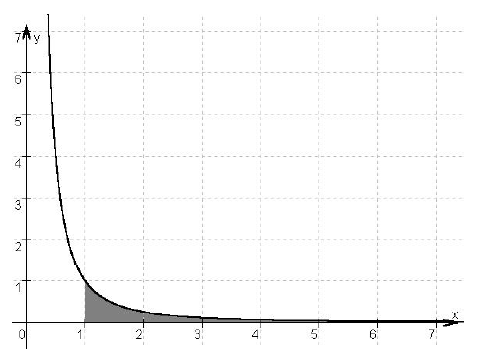
\includegraphics[width=0.6\linewidth]{images/images/Uneigentlicher_Integral_Beispiel1.png}
		\end{center}
	\end{minipage}
\end{definition}
\begin{KR}{Berechnung}
\begin{itemize}
	\item Rechnen mit endlichem Intervall \([a,\lambda] \text{ mit } \lambda \ge a \) anstelle von unendlichem
		Integral \([a,\infty) \)
		\[I(\lambda)=\int_a^{\lambda}{f(x)\mathrm{d}x} \]
	\item Das unendliche Intervall \([a,\infty) \) ergit sich aus \(\lim_{\lambda \rightarrow
		\infty}I(\lambda) \):
		\[I=\int_a^{\infty}{f(x)\mathrm{d}x}=\underset{\lambda \rightarrow \infty}{\lim}I(\lambda)=
		\underset{\lambda \rightarrow \infty}{\lim}\left(\int_a^{\lambda}{f(x)\mathrm{d}x}\right) \]
\end{itemize}
\end{KR}

\begin{KR}{Variante 1}
	\begin{itemize}
		\item Uneigentliche Integrale mit unendlichem Integrationsinvervall:
		\[I=\int_{-\infty}^b{f(x)\mathrm{d}x} \]
		\item Rechnen mit endlichem Invervall \([\lambda,b] \text{ mit } \lambda \le b \) anstelle von unendlichem
			Integral \((-\infty,b] \)
			\[I(\lambda)=\int_{\lambda}^b{f(x)\mathrm{d}x} \]
		\item Das unendliche Intervall \((-\infty,b] \) ergit sich aus \(\lim_{\lambda \rightarrow
			-\infty}I(\lambda) \):
			\[I=\int_{-\infty}^b{f(x)\mathrm{d}x}=\underset{\lambda \rightarrow -\infty}{\lim}I(\lambda)=
			\underset{\lambda \rightarrow -\infty}{\lim}\left(\int_{\lambda}^b{f(x)\mathrm{d}x}\right) \]
		\item Falls Grenzwert \(\underset{\lambda \rightarrow -\infty}{\lim}\) existiert, heisst das uneigentliche
			Integral \(\displaystyle\int_{-\infty}^b{f(x)\mathrm{d}x}\) \(\bold{konvergent}\), andernfalls 
			\(\bold{divergent}\)
	\end{itemize}
\end{KR}

\begin{KR}{Variante 2}
\begin{itemize}
	\item Uneigentliche Integrale mit beidseitig unendlichen Integrationsinvervall:
		\[I=\int_{-\infty}^{\infty}{f(x)\mathrm{d}x}\]
	\item Einfügen einer künslichen Zwischengrenze \(c \in \mathbb{R}\\\text{typischerweise}\:c=0 \)
		\[\int_{-\infty}^{\infty}{f(x)\mathrm{d}x}=\int_{-\infty}^{c}{f(x)\mathrm{d}x}+\int_c^{\infty}
		{f(x)\mathrm{d}x} \]
	\item Beide Teilintegrale wie oben berechnen
	\item Das integral heisst \(\bold{konvergent}\) falls beide Teilintegrale konvergent sind.
\end{itemize}
\end{KR}
\subsubsection{Uneigentliche Integrale zweiter Art}
	\begin{definition}{Definition}\\
		Uneigentlich Integrale auf Interval \([a,b]\) mit einem Pol von \(f(x)\) bei \(x=a\) heisst,
		\(f(a) \rightarrow \infty\), und Stetigkeit auf \((a,b]\)
		Graphische Darstellung:
	\begin{center}
		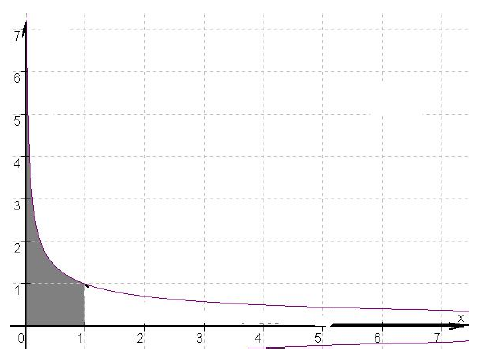
\includegraphics[width=0.4\linewidth]{images/images/Uneigentlicher_Integral_Beispiel2.png}
	\end{center}
  \end{definition}
  \begin{KR}{Berechnung}
	  \begin{itemize}
	  	
\item Statt über \([a,b]\) integrieren, integrieren über \(a+\epsilon,b\) für beliebige \(\epsilon>0\):
	\[I(\epsilon)=\int_{a+\epsilon}^b{f(x)\mathrm{d}x}\]
\item Das Integral über \([a,b]\) ergibt sich aus \(\lim_{\epsilon \rightarrow 0}I(\epsilon)\):
	\[I=\int_a^b{f(x)\mathrm{d}x}=\underset{\epsilon \rightarrow 0}{\lim}I(\epsilon)=\underset{\epsilon \rightarrow
	0}{\lim}\left(\int_{a+\epsilon}^b{f(x)\mathrm{d}x}\right) \]
\item Das Integral heisst \(\bold{konvergent}\), falls der Limes \(\lim_{\epsilon \rightarrow 0}I(\epsilon)\) existiert.
\item Diese spezielle Variante ist nötig, weil beim Integralrechnen der Integral auf dem ganzen Intervall stetig sein
	muss. Dies ist nicht der Fall wen ein Pol existiert.
\end{itemize}
  \end{KR}
